
\documentclass[margin, 11pt]{res} % Use the res.cls style, the font size can be changed to 11pt or 12pt here

\usepackage{helvet} 
\usepackage{multicol}
\usepackage{graphicx}
\setlength{\textwidth}{5.1in} % Text width of the document

\begin{document}

\moveleft.5\hoffset\centerline{\LARGE\bf Sorabh Rathod} % Your name at the top
 
\moveleft\hoffset\vbox{\hrule width\resumewidth height 1pt}\smallskip
 
\vspace{.05in}
{\large 
	7/32,Sarvodaya Estate,        \hspace{80pt}  
	Contact:  7977285338 \\
	Chembur, 
	\hspace{152pt}  
	e-mailid:  sorabh.r@somaiya.edu\\
	Mumbai - 400071,\\
	Maharashtra.\\
	
	\hspace{7.5cm}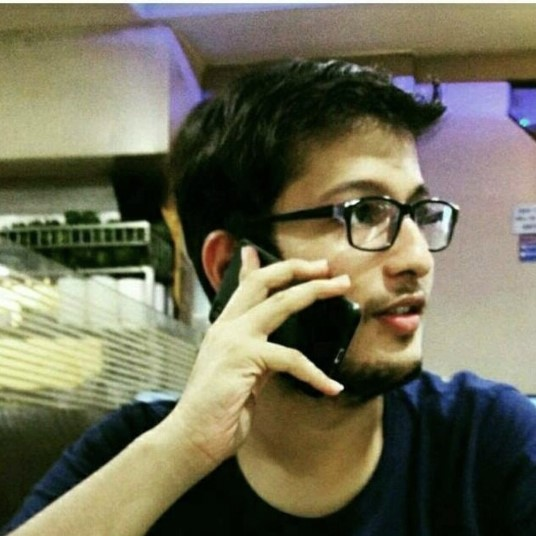
\includegraphics[height=3cm, width=3cm]{takephoto.jpg}\\
}


\begin{resume}


\section{OBJECTIVE \\ EDUCATION}  

\begin{tabular}{|c|c|c|c|c|}
	\hline
	Degree & College/School & University & Passing Year & Pass Percentage \\
	\hline
	SSC & Saraswati Vidyalaya & M.S.B.H.S.E & 2013 & 92.55 \% \\
	\hline
	HSC & Swami Vivekananda & M.S.B.H.S.E & 2015 & 91.09 \% \\
	\hline
	B.Tech & K.J.S.C.E & Mumbai University & 2019 & 9.45 GPA \\
	\hline
\end{tabular}

\vspace{.15in}
\section{PROJECTS} 

\begin{enumerate}
	\item Developed Disaster Detective Drone to find people trapped due to any natural calamity and help rescue them.
	\item Developed an Eco-Reflector for lights using shiny surface of plastic wrappers.
	\item Developed a prototype of car for handicap operating on timer using IC555.
	\item Developed a Solar Boiler with modification to enhance its performance.
	\item Project on comparison of performance of different Facial Recognition algorithms
	\item Accomplished line following using PID on lpc2148.
	\item Develpoed a robot being controlled via a webpage using RaspberryPi and Arduino, with access to registered user.
	\item Developed an android application for image recognition using IBM Waston API.
\end{enumerate}

\vspace{.15in} 
\section{TRAINING \& \\ INTERNSHIPS}

{\sl \textbf{Embedded Designer}} \hfill January 2018 - June 2018 \\
\textbf{Tortoise Learning} \\
\begin{itemize}
	\item Worked on development of embedded systems and made wireless robots for
	school students in order to give them an overview of robotics platform and how it
	can make lives easy.
	\item Developed a wireless soccer robot for the students to have robo soccer.
\end{itemize}

{\sl \textbf{Content Developer}} \hfill June 2018 \\
\textbf{Visha World} \\
\begin{itemize}
	\item Worked on content development of sensors like temprature sensor (DHT22), accelerometer and displays like TFT display, OLED display etc.
	\item Content included technical specifications of module and providing their sample arduino code with library of the module.
\end{itemize}

{\sl \textbf{Embedded Programmer}} \hfill June 2018 \\
\textbf{K.J.S.C.E} \\
\begin{itemize}
	\item Learned the basics of I2C protocol and established communication between two atmega 2560 boards. 
	\item Worked on interfacing of accelerometer with firebird V robot (ATmega 2560 board).
\end{itemize}

{\sl \textbf{Embedded Developer}} \hfill June 2018 - Present \\
\textbf{Cresla}\\
\begin{itemize}
	\item Worked with this company’s project based on agricultural purpose using Arduino
	and Raspberry Pi.
	\item Worked on framework like NodeRed for GUI development of project on RaspberryPi.
\end{itemize}


\vspace{.15in}
\section{TECHNICAL \\ SKILLS}

\begin{multicols}{2}
	\begin{itemize}
		\item Internet of Things (IoT)
		\item Arduino (Advanced)
		\item Atmel AVR
		\item Embedded Systems
		\item ARM Microcontroller
		\item Raspberry Pi
		\item MSP430
		\item Robotics
		\item AutoCad
		\item Hardware Debugging
		\item C Programming
		\item Java (Basics)
		\item Web Development (Basic)
		\item Node Red
		\item MATLAB
		\item Python
		\item MySQL Server
		\item Data Analysis using R
		\item Machine Learning
		\item Neural Networks
		\item Data Visualisation
	\end{itemize}
\end{multicols}


\vspace{.15in}
\section{SOFT SKILLS}

\begin{multicols}{2}
	\begin{itemize}
		\item Communication
		\item Clarity
		\item Confidence
		\item Listening
		\item Coordination
		\item Idea Exchange
		\item Team Management
		\item Optimism
		\item Self-motivation
		\item Decision making
		\item Experimenting
		\item Initiative
		\item Commitment
		\item Time-management
		\item Public speaking
		\item Observation
	\end{itemize}
\end{multicols}


\vspace{.15in}
\section{EXTRA-CURRICULAR \\ ACTIVITIES} 

Eyantra Robotics Competition, {\sl Team Leader} \hfill August 2016 - March 2017\\
Texas Innovation Challenge {\sl Team Leader} \hfill August 2018 - December 2018\\
Eyantra Robotics Competition, {\sl Team Leader} \hfill August 2018 - March 2019\\
 \\


\vspace{.15in}
\section{CO-CURRICULAR \\ ACTIVITIES} 

\begin{itemize}
	\item Represented department in Chess at inter-department sports event.
	\item Represented department in Carrom at inter-department sports event.
	\item Attended a workshop on MSP430 by Texas instrument.
	\item Represented department in Cricket at inter-department sports event.
	\item Attended a workshop on Internet of Things by ATS Learning Solutions. 
	\item Represented department in Badminton at inter-department sports event.\\
\end{itemize}


\vspace{.15in}
\section{Personal Details}

Father's name : Dharmendra Rathod. \\
Mother's name : Meena Rathod. \\
Sex : Male.\\
Date of Birth : 22 July, 1997.\\
Martial Status : Unmarried.

\vspace{.15in}
\section{Reference}

Vishwajit Parmar\\
CEO,\\
Cresla\\
Chembur,Mumbai.\\
98814 62555\\

Chandra Shekar\\
CEO,\\
Tortoise Learning\\
Madhya Pradesh.\\
89598 44865\\

Sachin Gala\\
Buisness Development Executive,\\
NJOY3D\\
Mumbai.\\
81087 96597\\[0.2mm]


\vspace{.15in}
\section{Declaration}

I hereby declare that above-mentioned information is correct to the best of my knowledge and belief


\vspace{.15in}
\section{Date} 

\date{\thedate}{\today}

\end{resume}
\end{document}